\chapter{Podłoże Pracy}
\section{Zachowanie organizmu w strefie śmierci Himalajów: Wpływ niskiego ciśnienia atmosferycznego na dostępność tlenu}
"Dead zone", znana również jako strefa śmierci, to obszar na dużych wysokościach górskich, gdzie ciśnienie atmosferyczne jest na tyle niskie, że ilość tlenu jest zbyt mała, by utrzymać życie. Przykładem takiej strefy jest tzw. "Death Zone" w Himalajach, znajdująca się powyżej wysokości około 8 000 metrów nad poziomem morza. W strefie śmierci organizm ludzki zaczyna doświadczać poważnych problemów związanych z niedoborem tlenu. Oto kilka głównych aspektów zachowania organizmu pod względem tlenu na wysokościach, zwłaszcza w obszarach dead zone:, niedotlenienie, objawy choroby wysokościowej, zmniejszona sprawność fizyczna, zespół cienkiego powietrza, ryzyko obrzęku mózgu i płuc. \cite{deathzone}

Z tego powodu himalaistom podejmującym wyzwania na obszarach dead zone zaleca się staranne przygotowanie fizyczne i aklimatyzację, a także świadomość własnego organizmu i objawów choroby wysokościowej. W przypadku dłuższego pobytu w takich warunkach, konieczne może być korzystanie z butli z dodatkowym tlenem, co pomaga złagodzić skutki niedoboru tlenu.

\section{Adaptacje układu krwionośnego w warunkach wysokogórskich}
Adaptacje układu krwionośnego w warunkach wysokogórskich są kompleksowymi zmianami fizjologicznymi, jakie zachodzą w organizmie w odpowiedzi na ekstremalne warunki panujące na dużych wysokościach. Poniżej opisano główne adaptacje układu krwionośnego \cite{adaptacja}, które występują w warunkach wysokogórskich: 
\begin{itemize}
    \item Zwiększenie liczby czerwonych krwinek (erytropoeza): Jedną z kluczowych adaptacji jest zwiększenie produkcji czerwonych krwinek w szpiku kostnym w odpowiedzi na niską dostępność tlenu na dużych wysokościach. To zjawisko, nazywane erytropoezą, ma na celu zwiększenie zdolności krwi do transportu tlenu.
    \item Zwiększenie hematokrytu: Hematokryt to odsetek objętości krwi zajmowanej przez czerwone krwinki. W warunkach wysokogórskich organizm może zwiększyć hematokryt, co pomaga w efektywniejszym przenoszeniu tlenu z płuc do tkanek.
    \item Zmniejszenie lepkości krwi: W odpowiedzi na hipoksję, organizm może zmniejszyć lepkość krwi, co ułatwia przepływ krwi przez naczynia w warunkach niskiego ciśnienia atmosferycznego.
    \item Zmniejszenie ciśnienia parcjalnego tlenu w płucach: Na dużych wysokościach, ciśnienie atmosferyczne jest niższe, co wpływa na ciśnienie parcjalne tlenu w płucach. To może prowadzić do zmniejszenia zdolności organizmu do nasycania krwi tlenem.
    \item Zwiększenie wentylacji płuc: W warunkach hipoksji organizm może zwiększyć tempo i głębokość oddechów w celu zwiększenia dostarczania tlenu do płuc.
    \item Regulacja przepływu krwi w narządach: W warunkach niskiego ciśnienia atmosferycznego organizm reguluje przepływ krwi w poszczególnych narządach, aby zaspokoić zwiększone zapotrzebowanie na tlenu w mięśniach i innych tkankach.
\end{itemize}

Te adaptacje pozwalają organizmowi lepiej radzić sobie z warunkami niskiego ciśnienia atmosferycznego i niedoboru tlenu na dużych wysokościach. Jednakże, istnieje indywidualna zmienność w zakresie adaptacji między różnymi osobami, a niektóre osoby mogą doświadczać problemów związanych z chorobą wysokościową, która wynika z trudności w dostosowaniu się do ekstremalnych warunków wysokogórskich.

\section{Pulsoksymetr, a wysokość}
Pulsoksymetr to przenośne urządzenie medyczne służące do pomiaru ilości tlenu we krwi oraz pulsu. Pulsoksymetr wykorzystuje dwa główne parametry do oceny stanu pacjenta: Saturacja tlenu (SpO2) - To procentowy stosunek tlenu do hemoglobiny we krwi. Pulsoksymetr mierzy stopień nasycenia krwi tlenem, co jest istotne dla monitorowania prawidłowego funkcjonowania układu oddechowego oraz puls - liczbę uderzeń serca na minutę. Ten parametr pomaga ocenić rytm serca i ogólną funkcję krążenia. Badania nad wynikami pulsoksymetru (SpO2) w kontekście zmieniającej się wysokości dostarczają istotnych informacji na temat adaptacji organizmu do ekstremalnych warunków górskich.

Obserwuje się tendencję do spadku poziomu SpO2 w miarę wzrostu wysokości \cite{spo2}. Istnieje znaczące zróżnicowanie między osobami w zakresie reakcji na zmiany wysokości. Niektórzy mogą utrzymywać stosunkowo stabilne wartości SpO2 w warunkach wysokogórskich, podczas gdy inni doświadczają znacznych spadków, co może wpływać na ich zdolność do funkcjonowania w trudnych warunkach. Badania sugerują, że spadek SpO2 może być związany z występowaniem objawów choroby wysokościowej, takich jak ból głowy, nudności czy ogólne osłabienie organizmu. Monitoring poziomu SpO2 może więc służyć jako wczesny wskaźnik potencjalnych problemów zdrowotnych na dużych wysokościach.

\begin{figure}[!htb]
    \centering
    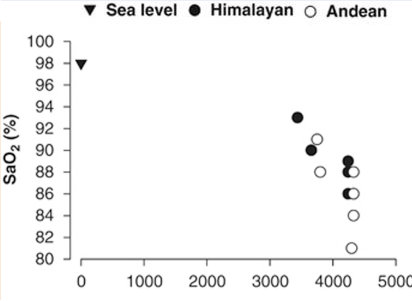
\includegraphics[width=.7\linewidth]{badaniaSPO2.png}
    \caption{Dane fizjologiczne pochodzące z 10 badań przeprowadzonych na wysokościach od 3658 do 4330 m. \cite{badaniaSPO2}}
\end{figure}